%Preamble
\documentclass[12pt,a4paper]{article}        %Define text type and basic formatting

\usepackage[utf8]{inputenc}     %Usage of UTF-8 for umlauts
\usepackage[ngerman]{babel}     %Paper language;
\pagenumbering{arabic}  % "Normal" page numbering
%Set line spacing to 1.5
\usepackage{setspace}
\onehalfspacing

%Citation and reference
\usepackage[backend=biber,
  style=authoryear,
  citestyle=authoryear-comp,
  hyperref=true,
  giveninits,    %Shorten first names to initial
  uniquename=init,    %prevent name disambiguation
  sorting=nyt,
  natbib  %enable citep/citet(parentheses only around year)
]{biblatex}   %REFERENCES https://www.overleaf.com/learn/latex/Bibliography_management_in_LaTeX
\addbibresource{references.bib}     %Lib file
\usepackage[nottoc,numbib]{tocbibind}   %add bibliography to toc

%page citation in text with colon: https://tex.stackexchange.com/questions/433122/changing-comma-in-textcite-to-colon
%\DeclareFieldFormat{postnote}{#1}
%\DeclareFieldFormat{multipostnote}{#1}
%\renewcommand\postnotedelim{\addcolon\addspace}
\renewcommand\nameyeardelim{\addcomma\space} %comma between author and year
%u.a. as et al.
\DefineBibliographyStrings{german}{%
  andothers = {et al.},
}
%Replace and/und with &
\renewcommand*{\finalnamedelim}{%
  \ifnumgreater{\value{liststop}}{2}{\finalandcomma}{}%
\addspace\&\space}%

%images
\usepackage{graphicx}       %Required for adding images
\graphicspath{{images/}}    %image path
\usepackage{wallpaper}  %Page background img

\usepackage{parskip}        %Prevent indention of paragraphs
\usepackage{mathtools}    %required for math formulas
\usepackage{amssymb}    %mathematical symbols
\usepackage{listings}   %For code listings

%Use markdown in LaTex https://de.overleaf.com/learn/latex/Articles/How_to_write_in_Markdown_on_Overleaf
\usepackage[footnotes,definitionLists,hashEnumerators,smartEllipses,hybrid]{markdown}

\usepackage{titlesec}   %Style titles
\usepackage{fancyhdr}   %Header/footer
\usepackage[bottom]{footmisc}   %Foot notes, at end of page

%Links
\usepackage[colorlinks,
  pdfpagelabels,
  pdfstartview = FitH,
  bookmarksopen = true,
  bookmarksnumbered = true,
  linkcolor = black,
  plainpages = false,
  hypertexnames = false,
  citecolor = black,
urlcolor = black]{hyperref}   %Hyperref pkg -> clickable links and TOC
\usepackage{csquotes}   % Autostyle quotes language-specific

%Font settings
\renewcommand{\familydefault}{\sfdefault}       %Text sans-serif
\renewcommand{\headrulewidth}{0pt}
\pagestyle{fancy}

%Footer
\fancyhf{}      %Clear all header/footer stylings
\lfoot{\thedate\hspace{1pt}}
\cfoot{Proposal Bachelorarbeit\\«Video- und bildbasierte Desinformation auf Social-Media-Plattformen in der Schweiz» (Arbeitstitel)}
\rfoot{\thepage\hspace{1pt}}        %Add page number

%Title page settings
\usepackage{pdfpages}
\usepackage{titling}    %Title page styling
\title{«Video- und bildbasierte Desinformation auf Social-Media-Plattformen in der Schweiz» (Arbeitstitel)}        %Document Title
\author{Yannick Spriessler}     %Author of paper
\date{07.02.2025}     %Date of paper; ALTERNATIVE: \today

% Separate bibliography for images
% \defbibheading{imagecredits}{\section*{Bildverweis}}
% \addbibresource{img-references.bib}

%___________________________________________________________________________________________
%TITLE PAGE
\begin{document}
\begin{titlingpage} %Start titling page
  % \begin{center}
  %   \begin{large}
  %     Fachhochschule Graubünden\\ Institut für Multimedia Production (IMP)\\ %The name of your university
  %   \end{large}
  %   \vspace{2cm} %You can control the vertical distance
  %   \begin{LARGE}
  %     \textbf{\thetitle} \\
  %   \end{LARGE}
  %   \vspace{1cm}
  %   \begin{large}
  %     Proposal Bachelorarbeit\\
  %   \end{large}
  %   \vspace{5cm} %Put the distance you need.
  %   Autor: \theauthor \\
  %   Studiengang: BSc Multimedia Production \\
  %   Matrikel-Nr.: 22-160-360 \\
  %   Adresse: Breitenstrasse 26, 4416 Bubendorf \\
  %   E-Mail: yannick.spriessler@stud.fhgr.ch \\ \\
  %   Referentin: Prof. Dr. Franziska Oehmer-Pedrazzi \\
  %   Koreferent: Benjamin Hanimann \\ \\
  %   Datum: \thedate
  % \end{center}
  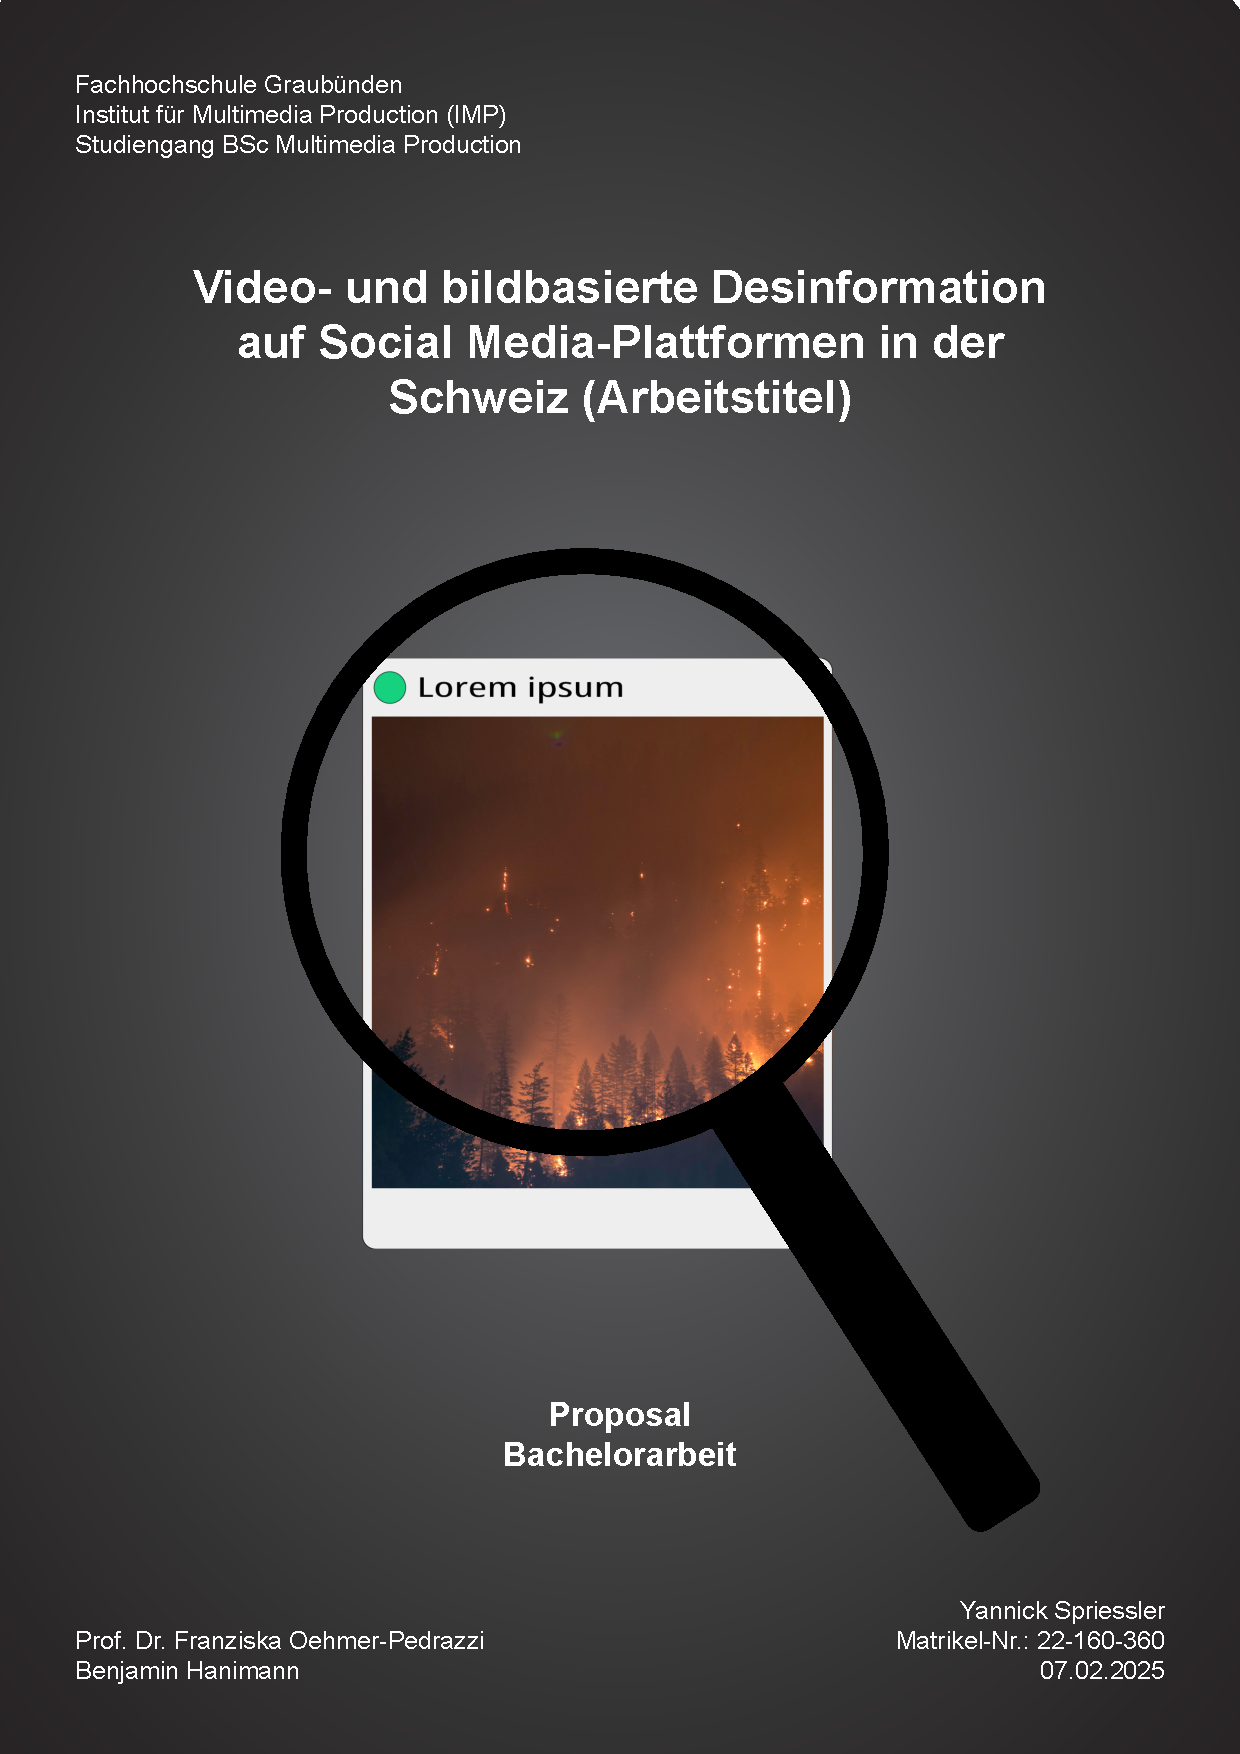
\includepdf{Titelblatt_Proposal}
  % {\small \phantom{Image courtesy of \cite{howard_trees_2017}.}}
\end{titlingpage}
\pagebreak      %Insert page break
%-----------------------------------------------
%TOC
\thispagestyle{empty}
\setcounter{page}{0}    %Set page no.
\tableofcontents        %Content index
\pagebreak
%-----------------------------------------------
%DOC
%\begin{abstract} \end{abstract}    %If abstract is used

%\frontmatter   %If foreword
%\mainmatter    %Main part if foreword used
\section{Thema}
Die Bachelorarbeit befasst sich damit, wie Inhalte auf Social-Media-Plattformen in der Schweiz verwendet werden, um durch video- und bildbasierte Desinformation politische oder gesellschaftliche Narrative zu stärken. Im anschliessenden Lehrprojekt werden diese Erkenntnisse verwendet, um darauf basierend eine interaktive Aufklärungsplattform zu gestalten.

\subsection{Meine Motivation}

Schon länger interessiere ich mich für Politik und gesellschaftliche Themen, aber auch für die technischen Aspekte von Social-Media-Plattformen. Durch meine Tätigkeiten als Leiter in diversen Jugendarbeits-Angeboten liegen mir Jugendliche und junge Erwachsene am Herzen, gleichzeitig bekomme ich bei ihnen hautnah mit, welchen Einfluss Social Media im Alltag hat, und auch ich selbst hinterfrage immer wieder meinen Umgang damit. \\
Ich bin der festen Überzeugung, dass eine mündige Gesellschaft darauf angewiesen ist, wahre von unwahren Tatsachen zu unterscheiden, um sich so eine fundierte Meinung bilden zu können, basierend auf Fakten und eigenen Werten, welche unter anderem auf diesen Fakten basieren. Deshalb möchte ich mit meiner Bachelorarbeit dazu beitragen, dass diese Kompetenz gestärkt werden kann.

\subsection{Zielsetzung \& Fragestellung der Bachelorthesis}
In meiner Bachelorarbeit setze ich mich mit der Fragestellung auseinander, welche inhaltlichen und gestalterischen Merkmale Desinformation auf Social-Media-Plattformen in der Schweiz aufweist. 

Ziel der Arbeit ist es zum einen herauszufinden, ob es mögliche Muster und Strategien hinter der Produktion der Inhalte gibt. Zum anderen soll auch ein allgemeines Verständnis über die entsprechenden Inhalte gewonnen werden.

\subsection{Zielsetzung Lehrprojekt}
Das Lehrprojekt soll als interaktive Aufklärungsplattform die Erkenntnisse aus der theoretischen Thesis aufgreifen und multimedial vermitteln. Dabei werden sowohl webbasierte, als auch videobasierte Formate eingebaut. \\

\section{Mediales Lehrprojekt}
\subsection{Form und Inhalt}
Als Lehrprojekt ist eine interaktive, webbasierte Aufklärungsplattform angedacht. Sie soll auf spannende und interaktive Art das Bewusstsein für die Verbreitung von Desinformation auf Social-Media-Plattformen stärken und Möglichkeiten vermitteln, diese besser zu erkennen und ihre Verbreitung einzudämmen.\\

\subsection{Konzept}
Umgesetzt werden soll die Plattform mit interaktiven Elementen und Videobeiträgen von Expertinnen und Experten. Als Beispiel dienen Plattformen wie \href{https://www.der-newstest.de}{Der Newstest.de} und \href{https://madetomeasure.online/de/}{Made To Measure}.\\
Zielgruppe sind alle Nutzenden von Social-Media-Plattformen, auf welchen entsprechende Inhalte verbreitet werden.

Der Fokus des Lehrprojekts liegt auf der interaktiven und zielgruppengerechten Kommunikation der wissenschaftlichen und gesellschaftsrelevanten Erkenntnisse. Durch das Lehrprojekt soll die Aufmerksamkeit der Nutzenden für desinformative Inhalte gesteigert werden. \\
Denkbar ist diesbezüglich auch eine Zusammenarbeit beispielsweise mit einem Lehrmittelverband oder Debunking-Plattformen wie Correctiv Schweiz. Dadurch können allenfalls weitere Bedürfnisse an eine solche Plattform abgeholt werden.

Geplant ist eine Umsetzung mit dem Vue-/Nuxt-Framework als Grundlage für die Webplattform. Videoinhalte werden auf YouTube gehostet und entsprechend eingebunden.\\
Informative Inhalte und Ergebnisse aus der schriftlichen Thesis wechseln sich ab mit ergänzenden und einordnenden Videoinhalten von Expertinnen und Experten. Diese werden während der Auswertungsphase und der Schreibphase produziert und können inhaltlich auch in die Thesis einfliessen.

\section{Bachelorthesis}
\subsection{Thema und Problemstellung}
Inhalte mit Schweizer Bezug, welche von Faktencheck-Plattformen aus dem DACH-Raum als Desinformation anerkannt wurden, werden durch eine Inhaltsanalyse strukturell untersucht, um daraus Erkenntnisse über oft verwendete Mechanismen bei ihrer Gestaltung zu gewinnen. Diese werden danach verwendet, um darauf basierend als Lehrprojekt eine interaktive Aufklärungsplattform für Nutzende dieser sozialen Plattformen zu gestalten.

Um das Problem um Desinformation auf Social Media besser zu verstehen, wird im Theorieteil der Arbeit ausserdem auch auf die Funktionsweise der Plattformen und ihre Algorithmen (sofern bekannt) eingegangen sowie auf die Problemstellungen durch generative künstliche Intelligenz und allfällige Eindämmungsmöglichkeiten gegen die Verbreitung von Desinformation.

\subsection{Relevanz}

\subsubsection{Gesellschaft}
Im Jahr 2024 betrug der Anteil der Social-Media-Nutzenden in der Schweiz knapp 80\% \parencite[22]{we_are_social_anteil_2024}. Somit wird durch Social-Media-Inhalte ein Grossteil der Schweizer Bevölkerung erreicht. Dadurch kann Desinformation potenziell einen grossen Einfluss auf die Bevölkerung und ihre (politische) Meinungsbildung haben \parencites[18]{grujic_warnhinweise_2024}[258]{hohlfeld_schlechte_2020}[1]{khan_fake_2021}. \\
\textcite[258]{hohlfeld_schlechte_2020} schreiben Desinformation die Fähigkeit zu, demokratische Gesellschaften “durch Inhalte, die Angst und Verunsicherung schüren, [...] durch die Schwächung der seriösen Institutionen der Erkenntnisbeschaffung und [...] durch Normverschiebungen des politisch Sagbaren” zu destablisieren. Gemäss dem \textcite{bundesministerium_des_innern_und_fur_heimat_desinformation_2022} (zit. nach \textcite[15]{teetz_Social Media-post_2023}) kann Desinformation ab einem gewissen Grad sogar als Bedrohung der nationalen Sicherheit verstanden werden.

\subsubsection{Wissenschaft}
Social-Media-Plattformen und ihre entsprechenden Algorithmen zur Inhaltsauswahl basieren neben den Interaktionen der Nutzenden untereinander in ihrer Funktionsweise vor allem auf der Generierung von Aufmerksamkeit \parencites[vgl.][220]{schmidt_meinungsbildung_2022}[493]{behnke_manipulation_2018}. Durch die Verbreitung eines Inhaltes wird zwangsläufig die Kapazität der Nutzenden für die Verarbeitung anderer Inhalte geschmälert \parencite[248]{hohlfeld_schlechte_2020}. \\
Die Wissenschaft kennt das Potenzial und die Gefahr von Social-Media-Plattformen, durch Fragmentierung und das Anzeigen bestimmter Inhalte Filterblasen zu schaffen und die Gesellschaft zu spalten – dieser Effekt konnte jedoch bisher nicht tatsächlich bewiesen werden \parencite[220]{schmidt_meinungsbildung_2022}.\\

Demokratische Meinungsbildung erfordert Kenntnis über die korrekte Faktenlage. Durch das Wissen über die Mechanismen der Social-Media-Plattformen und die Fähigkeit, falsche von echten Tatsachen zu unterscheiden, kann die Gefahr verringert werden, dass durch Desinformation und bewusst provozierte Narrative die eigene Meinungsbildung beeinflusst wird.\\
Meine Arbeit hat zum Ziel, über Desinformation aufzuklären und ein grösseres Bewusstsein dafür zu schaffen, damit sich bestenfalls ihr Einfluss auf die Meinungsbildung der Schweizer Bevölkerung verringert.

\subsection{Forschungsfrage}
Folgende Fragestellung wird in der Bachelorarbeit behandelt:\\

\begin{quote}
  Welche inhaltlichen und gestalterischen Merkmale weist video- und bildbasierte Desinformation auf Social-Media-Plattformen in der Schweiz auf?
\end{quote}

\subsection{Forschungsstand}

Bei Desinformation handelt es sich nach \textcite[213]{allcott_social_2017} um "[...] news articles that are intentionally and verifiably false, and could mislead readers." \textcite{marx_fake_2020} definieren aktuelle Desinformation als "Kommunikation wissentlich und empirisch falscher Informationen zu neuen und relevanten Sachverhalten mit dem Anspruch auf Wahrheit." \\
Die Motivation hinter Desinformation umfasst normalerweise entweder finanzielle oder ideologische Zwecke \parencites[vgl.][138]{tandoc_defining_2018}[225]{schmidt_meinungsbildung_2022}[154-155]{lange_unsicherheit_2019}.

Der Begriff "Fake News" wurde zunehmend zu politischen Propagandazwecken verwendet. \Textcite[148]{marx_fake_2020} empfehlen deshalb, stattdessen von aktueller Desinformation zu sprechen. \\
Bezüglich den Definitionskriterien für Desinformation besteht in der Wissenschaft Uneinigkeit; die folgende Arbeit stützt sich deshalb auf die Kriterien nach \textcite{marx_fake_2020}: \\
- (Visuelle) Kommunikation \\
- Aktualitätsbezug \\
- Wahrheitsanspruch in Abgrenzung zur Satire \\
- Unwahrheit: Irreführendes Potenzial \\
- Unwahrhaftigkeit: Die Produzierenden sind sich der Unwahrhaftigkeit ihrer Nachricht bewusst \\
- Täuschungsabsicht: Vorsätzliche Verbreitung falscher Tatsachen\\

Desinformation dient in der Regel dazu, politische Ziele zu erreichen, das Vertrauen in öffentliche Institutionen zu schmälern und die Polarisierung der Gesellschaft voranzutreiben \parencites[vgl.][ ]{allcott_social_2017}[225]{schmidt_meinungsbildung_2022}[162]{lange_unsicherheit_2019}. \\

In Anlehnung daran kann davon ausgegangen werden, dass Desinformation gemäss den oben definierten Kriterien vermutlich vor allem im politischen Kontext betrieben wird \parencites[vgl.][51]{sammer_fake_2021}[217]{allcott_social_2017}[498]{behnke_manipulation_2018}. Eine klare Absenderschaft lässt sich jedoch meist nur schwer definieren \parencite[498-499]{behnke_manipulation_2018}.

\subsection{Methodik}
Methodisch ist eine Inhaltsanalyse aktueller video-/bildbasierter Desinformation auf Social-Media-Plattformen in der Schweiz geplant. Dazu werden Inhalte untersucht, welche von Faktencheck-Plattformen im entsprechenden Gebiet als Desinformation markiert wurden. \\
Des Weiteren sind zur Einordnung und zugunsten weiterer Erkenntnisse Experteninterviews geplant, welche dann in Videoform gegebenenfalls auch für das Lehrprojekt verwendet werden.

\subsubsection{Analysegegenstand}
Diverse Faktencheck-Plattformen publizieren ihre Erkenntnisse zu geprüften Inhalten online. Die untersuchten Artefakte sowie die Artikel dazu werden strukturiert ausgewertet, um daraus möglichst Mechanismen für Desinformation auf Social Media abzuleiten. Durch die Limitierung auf solche Plattformen kann sichergestellt werden, dass entsprechende Kriterien für die Qualifikation als Desinformation der Inhalte gegeben sind.

\subsubsection{Datenerhebung und Auswertungsmethode}
Die Datenerhebung geschieht mittels eines selbstprogrammierten Python-Webcrawlers, welcher sämtliche Artikel der Faktencheck-Plattformen im festgelegten Zeitraum ausliest und in einer geeigneten Datei speichert. \\
Die Daten werden anschliessend durch eine standardisierte, quantitative und qualitative Inhaltsanalyse ausgewertet. Neben quantitativen Metadaten (bspw. Veröffentlichungsdatum des Artikels, welcher Aufschluss gibt über den Zeitraum, in welchem die Desinformation verbreitet wurde) sind weitere Codierungen erforderlich, um die Inhalte auch qualitativ auszuwerten. Denkbar wären hier beispielsweise Auswertungen zu den behandelten Themen, den Verbreitungsplattformen und weitere.

\subsubsection{Analysezeitraum}
Untersucht werden Beiträge zu Inhalten ab 2020. So wird einerseits deren Aktualitätsbezug sichergestellt, andererseits wird in Krisenzeiten nachweislich besonders viel Desinformation verbreitet (\textcite{tandoc_defining_2018} zit. nach \textcite[2]{ceron_fake_2021}). Dies lässt sich auch für die Covid19-Pandemie nachweisen (ebd.).

Spannend wird in diesem Zusammenhang ausserdem sein, ob durch den KI-Boom in diesem Zeitraum ein Anstieg von Desinformation zu verzeichnen ist. \textcite[e32-3]{bontridder_role_2021} legen dar, wie mit künstlicher Intelligenz zum einen neue Manipulationsarten (bspw. Deepfakes) zur Verfügung stehen, und zum anderen, wie auf KI basierende Algorithmen signifikant zu deren Verbreitung beitragen.
Dieser potenzielle Anstieg wird gemessen anhand des Veröffentlichungsdatums der Untersuchungen durch die Faktencheck-Plattformen.


\subsection{Darstellung Grobstruktur der Arbeit}
Link zur aktuellen Gliederung (Notion-Page): \href{https://yannix.notion.site/Vorl-ufige-Gliederung-132c91f07039801fb0e0ed859201268b}{Vorläufige Gliederung}

\section{Zeitplan}
Siehe Anhang.

\section{AI-Tools}
Es wurden keine AI-Tools zum Schreiben des Proposals verwendet.

\pagebreak
%-----------------------------------------------
%BIB
\section{Literaturverzeichnis}

\subsection{Weitere mögliche Quellen}

- \cite{antos_web_2019} \\
- \cite{bontridder_role_2021} \\
- \cite{brill_death_2024} \\
- \cite{fernandes_post-factual_2022} \\
- \cite{kertysova_artificial_2018} \\
- \cite{latzer_vertrauen_2023} \\
- \cite{montasari_artificial_2022} \\
- \cite{reuter_fake_2019} \\
- \cite{wahl_fake_2021} \\
- \cite{dander_fake_2020} \\
- \cite{waller_jamesfocus_2019} \\
- \cite{zoglauer_konstruierte_2021} \\

\printbibliography
% \section {Bildverweis}
% \printbibliography[heading=imagecredits, keyword=image]
\end{document}
